\documentclass[Rapport/Rapport_main.tex]{subfiles}
\begin{document}
\section{Analyse}
I dette afsnit beskrives resultater af analysen. De største overvejelser for projektet har omhandlet den grafiske brugeroverfalde og databasen. De endelige valg begrundes kort for applikationen og databasen. for den fulde analyse henvises til bilaget \textbf{Analyse}.

\subsection{Applikationstype}
Det var et krav for systemet, at det skulle være en applikation, der kun interagere med brugere gennem en grafisk brugeroverflade. Der var tale om flere typer applikationer, samt hvorvidt den skulle være platformsuafhængig. WPF systemet blev valgt efter dets MVVM-struktureret design passede til vores behov, samt det gav et system med lav kobling mellem de forskellige lag (Presentation, Business og Data layer). Desuden var frameworket en del af pensum, hvilke betød at der var rig mulighed for hjælp af faglærere. 
\subsubsection{MVVM}
MVVM arkitekturen gør det muligt at holde applikationens forretnings- og præsentationslogik adskilt. Arkitekturen består af tre kernekomponenter: View, ViewModel og Model (se figur \ref{fig:MVVM_pic}) \\\\
\begin{figure}[H]
    \centering
    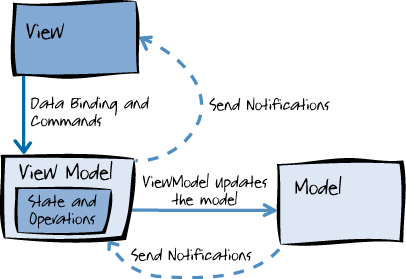
\includegraphics[width=0.90\textwidth]{Rapport/Analyse/graphics/MVVM.png}
    \caption{MVVM arkitektur\cite{MVVM}}
    \label{fig:MVVM_pic}
\end{figure}
\textbf{Views} indkapsler brugeroverflade og dets logik. View'et er de visuelle elementer, som præsenteres for brugeren. \\\\
\textbf{ViewModels} indholder præsentationslogikken og dets stadie. Det har ingen direkte reference til View'et. ViewModellen indeholder properties og kommandoer, som databindes til View'et. View'et bestemmer, hvordan funktionalitetet skal gengives, hvor ViewModeller har til ansvar at koordinere View'ets interaktion med systemets data og modeller\\\\
\textbf{Modeller} indeholder applikationens forretningslogik og -data. Dette kan være hentning og administration af applikationsdata og for at sikre at forretningsregler, der sikrer datakonsistens og -gyldighed, bliver overholdt. 

\subsection{Database}
For at kunne opbevare brugerdata, er det nødvendigt at have en database. Hertil blev der overvejet to forskellige løsninger: En lokal database eller administreret clouddatabase. Den lokale database krævede at der konstant skulle have en computer/enhed stående, som holdte databasen aktiv (Det er ikke let at distribuere en relationel database ud på flere maskiner). Microsoft Azure SQL database udbyder et administreret clouddatabase system, og tilbyder studerende 2GB hukommelse i et givet tidsinterval. Desuden er Azure også indbygget i Visual studio, hvilke er det IDE, som de fleste i gruppen bruger. \\
Det er valgt at lave en relationel database, da NOSQL er optimeret mere mod store mængder data af varierende type og mindre mod garantier for at data er fejlfri. Siden vi arbejder med relativt små mængder data som involvere personlig info er det vigtigere at data er garanteret for at være korrekt. Desuden understøøer Microsoft Azure ikke NOSQL.

Analysen af systemet har reduceret design valgene for projektet ud fra de ressourcer og funktionalitet, som er blevet prioriteret. Som det første planlægges arkitekturen for systemet. 
\end{document}